\documentclass[main.tex]{subfiles}

\begin{document}
	
\section{Pomer dĺžky najkratšej cesty v sieti a vzdialenosti vzdušnou čiarou}
\label{sec:random_paths}

V tejto časti porovnávame efektívnosť železničných sietí na Slovensku a v Českej republike. Naša hypotéza predpokladá, že nižšia prepojenosť slovenskej siete spôsobuje, že cestujúci musia častejšie využívať nepriame trasy, čo vedie k vyššiemu pomeru dĺžky najkratšej cesty v sieti k priamej vzdialenosti medzi stanicami v porovnaní s českou sieťou.

Na overenie hypotézy sme použili stochastický prístup. Náhodne sme vyberali dvojice staníc a určovali najkratšiu cestu v sieti na základe váh hrán reprezentujúcich vzdialenosti. Túto dĺžku sme porovnali s priamou vzdialenosťou medzi stanicami, vypočítanou pomocou ich geografických súradníc, a vypočítali pomer týchto dvoch hodnôt.

Stanice sme nevyberali uniformne náhodne, ale vážili sme ich podľa počtu obyvateľov obcí, ku ktorým patria, aby sme lepšie odrážali reálne cestovné vzorce – väčšie mestá sú častejšími cieľmi. Ak jedna obec mala viacero staníc, počet obyvateľov sme rozdelili proporčne. Staniciam, ktoré nebolo možné priradiť k obci, sme priradili defaultnú hodnotu 1000 obyvateľov. Následne sme normalizovali počty obyvateľov, aby sme získali pravdepodobnostné rozdelenie. Celkový počet obyvateľov použitý pre Slovensko bol 3\,096\,147 a pre Česko 7\,179\,048.

Na ilustráciu náhodného výberu dvojice staníc sme zvolili príklad zo Slovenska, znázornený na obrázku~\ref{obr:svk_skyline_vs_shortest}. Spojenie medzi stanicami Kokava nad Rimavicou a Spišská Nová Ves, ktoré sú geograficky relatívne blízko, ukazuje značnú neefektívnosť železničnej siete. Najkratšia cesta železnicou je 3,8-krát dlhšia ako priama vzdialenosť vzduchom, čo poukazuje na obmedzenú prepojenosť siete v tejto oblasti.

Simuláciu sme pre obe krajiny spustili 1 milión krát. Výsledky simulácie sú zhrnuté v tabuľke~\ref{tab:ratios}.

\begin{table}[H]
\centering
\begin{tabular}{|l|c|c|}
\hline
 & Slovensko & Česká republika \\
\hline
Priemerný pomer & 1.7941 & 1.3394 \\
Medián pomeru & 1.3172 & 1.2710 \\
Maximálny pomer & 375.0649 & 38.3310 \\
\hline
\end{tabular}
\caption{Porovnanie pomerov dĺžok ciest medzi stanicami}
\label{tab:ratios}
\end{table}

Na Slovensku sme zaznamenali extrémny pomer 375.0649 medzi stanicami Bratislava predmestie a Bratislava - Vinohrady, čo je reálny príklad dané stanice sú vzdialené pár metrov ale keďže nie je medzi nimi spojenie ukazujú sa ako veľky outlier. Takýto typ dvoch vybratých staníc avšak nie je veľa. Je jasné, že prepojenie daných dvoch staníc by nepomohlo infraštruktúre. V Českej republike dosiahol maximálny pomer 38.3310 medzi stanicami Rychnov nad Kněžnou a Vamberk, no tento prípad je nereálny kvôli chybe v dátach (neexistujúca hrana), aj napriek snahe o zachytenie všetkých nekonzistentností sme stále v českých dátach našli chybajúce hrany. 


Výsledky avšak potvrdili našu hypotézu: priemerný pomer je na Slovensku vyšší (1.7941) ako v Českej republike (1.3394), čo naznačuje, že cestujúci na Slovensku častejšie musia voliť nepriame trasy. Pri zohľadnení nekonzistentnosti Českých dát je výsledok ešte horší slovesnkú infraštruktúru, keďže chýbajúce hrany spôsobujú zvýšenie pomeru. Ak by sme zohľadnili aj priemerné rýchlosti vlakov, rozdiel v neprospech slovenskej infraštruktúry by bol pravdepodobne ešte výraznejší.

\begin{figure}
\centerline{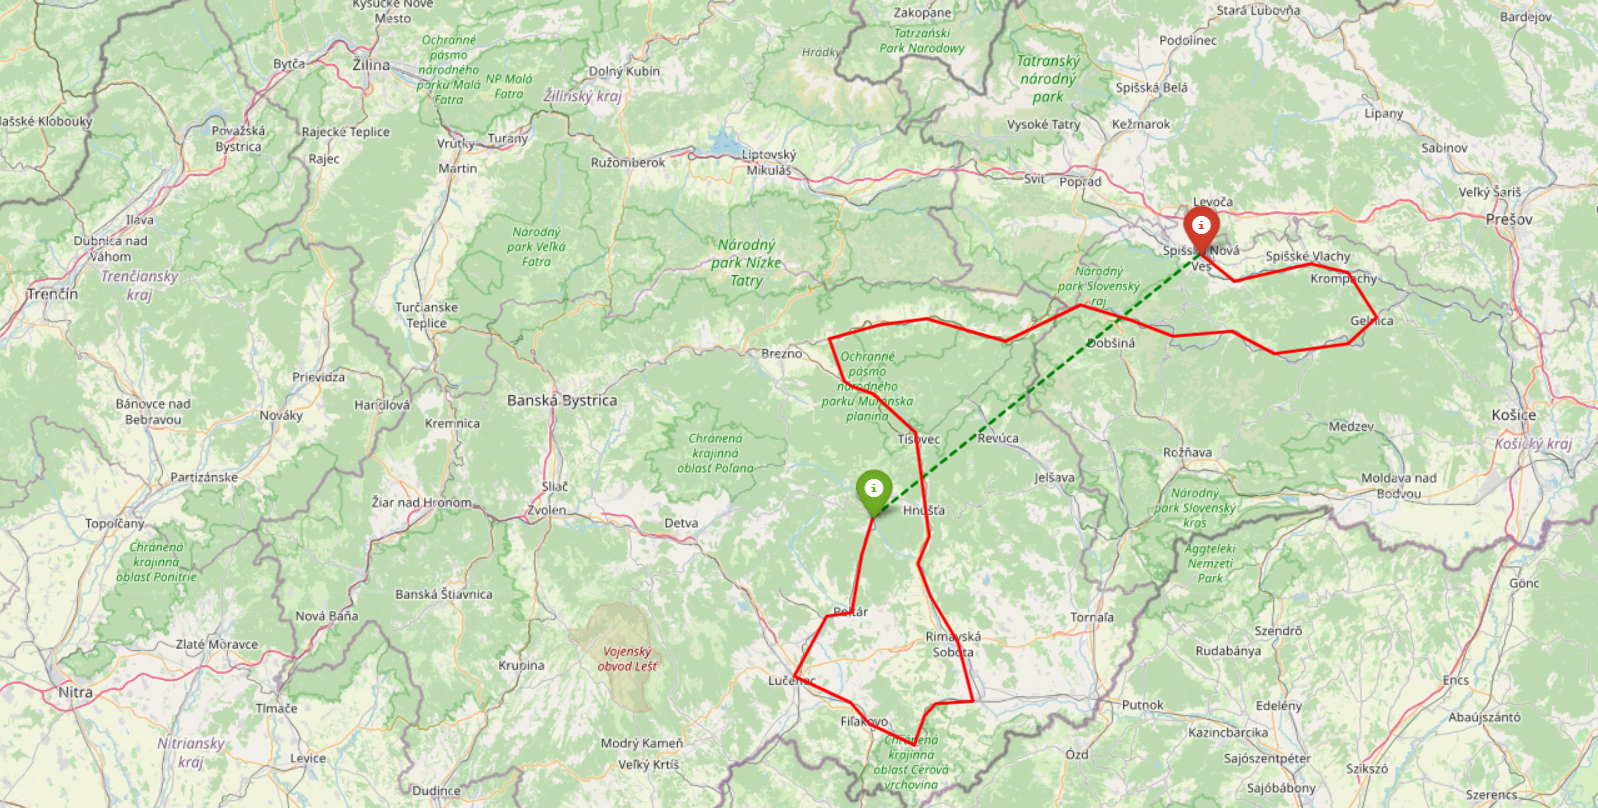
\includegraphics[width=1.2\textwidth]{images/sk_shortest_path_vs_skyline.png}}
\caption{Príklad dvojice staníc a porovnania najkratšej trasy v železničnej sieti a vzdielenosti vzdušnou čiarou}
\label{obr:svk_skyline_vs_shortest}
\end{figure}

